\documentclass{article}

\usepackage[left=2.5cm, right=2.5cm,top=2.5cm, bottom=2.5cm]{geometry}

\usepackage{physics}        % Braket and more
\usepackage{siunitx}        % Writing SI-units
\usepackage{amsmath}        % Fancy math
\usepackage{tikz}           % Drawing
\usepackage{graphicx}       % Figures
\usepackage{algorithm}      % Writing code
\usepackage{algpseudocode}
\usepackage{subcaption}

\graphicspath{{./figs/}}


\title{Simulation of time dependent hamiltonian}
\author{Martin Johnsrud}
\date{}

\begin{document}

\maketitle
\begin{abstract}
    this is an abstract
\end{abstract}

\section*{Parametres}

    The 1D time dependent Schrödinger equation is given by

    \begin{equation*}
        \hat H \Psi(x, t) = i \hbar \pdv{t} \Psi(x, t), \quad \hat H = -\frac{\hbar}{2m}\pdv[2]{x} + V(x, t),
    \end{equation*}

    for some potential $V(x)$. However, it is cumbersom to walk with dimensonfull constants, especially numerically, when values for $\hbar$ in the si-system is of order $10^{-34}$. This can lead to inaccuracies when doing numerical simulations. But, by choosing some defining, problem-dependent sizes and grouping togheter the constants, this can be liminated by the introduction of dimensonless variables. We are going to be working with potentials which are infinit outside som local region, i.e. the boundary conditions $\psi(0>x>L) = 0$, so it is natural to choose the length of the potential, $L$, as a defining quantity. Noticing that

    \begin{equation*}
        \bigg[\frac{\hbar}{2 m L^2} \bigg] = \frac{\si{kg.m^2.s^{-1}}}{\si{kg.m^2}} = \si{s^{-1}},
    \end{equation*}
    we make the variable change
    \begin{equation*}
        \frac{\hbar}{2 m L^2}t \rightarrow t, \quad \frac{1}{L}x \rightarrow x.
    \end{equation*}
    This gives the new, dimensionless schrödinger equation
    \begin{equation}
        \hat H \Psi(x, t) = -i \pdv{t} \Psi(x, t), \quad \hat H = -\pdv[2]{x} + V(x, t),
        \label{time_depend}
    \end{equation}
    where I have done the change $2mL/\hbar^2V(x, t) \rightarrow V(x, t)$. All sizes now is in units defined by the problem and the constants of the equation, and the new boundary condition is 
    \begin{equation*}
        \Psi(0>x>1) = 0.
    \end{equation*}

\section*{Time independent problems}
    Assuming, for now, that the potential is independent of time, we can get the time independent schrødinger equation from \eqref{time_depend} by separation of variables. Assuming $\Psi(x, t) = \psi(x)\phi(t)$  yields the time independent schrödinger equation and the equation for the time dependence:
    \begin{equation}
        \bigg[-\pdv[2]{x} + V(x) \bigg] \psi(x) = \hat H \psi = E \psi(x), \quad \pdv{t}\phi(t) = -iE\phi(t).
        \label{TUSL}
    \end{equation}
    The equation for time is elematary, and gives the solution $\phi(t) = \exp(-iEt)$. The time independent schrödinger equation is a eigenvalue problem, and can be solved by discretizing the hamiltonian, and thus also $\psi$. 
    \begin{equation*}
        \pdv[2]{x}\psi(x) = E \psi(x).
    \end{equation*}
    Using a finite difference scheme with $N + 1$ nodes, there will be $N-1$ possibly non-zero nodes. The end node are given by the boundary conditions $\psi(0) = \psi(1) = 0$, and the interior points are given by the matrix equation
    \begin{equation*}
        H \psi_n = E_n \psi_n, \quad H_{ii} = 2N^2 + V_i, D_{ii\pm1} = -N^2.
    \end{equation*}
    Here, $\psi_n$ is a vector such that $\psi_n^{(i)} = \psi_n\big((i+1)/N\big)$, and $V_i$ is the potential evaluated at that node. This is shown in the figure bleow.

    \begin{center}
    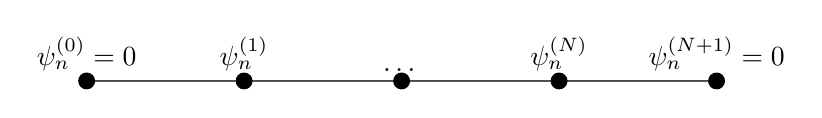
\begin{tikzpicture}
        \filldraw
        (0, 0) circle (0.1) node[align=center, above] {$\psi_n^{(0)} = 0$}--
        (2, 0) circle (0.1) node[align=center, above] {$\psi_n^{(1)}$}--
        (4, 0) circle (0.1) node[align=center, above] {\dots} --
        (6, 0) circle (0.1) node[align=center, above] {$\psi_n^{(N)}$}--
        (8, 0) circle (0.1) node[align=center, above] {$\psi_n^{(N+1)} = 0$};
    \end{tikzpicture}
    \end{center}

\subsection*{Particle in a box}
    The method is first tested at a particle in a box, i.e. $V(0<x<1) = 0$. The result of the simulation, togheter with the analytical solution, is shown in figure \ref{fig:particel in box}. The normalization is such that the sum ${\psi_n^{j}}^\dagger\psi_n^{j} = 1$ holds. The analytical solution for the eiegenvalues are $E_n = (n \pi)^2$. By the finite nature of this simulation, the values are going to be less accurate for the higher energies, as they are waves where the wave length is short, and is aproaching the resolution of the discretization. Figure \ref{fig:eigenvalues} shows the numerically computed eigenvalues, and compares them to the analytical solution. We see the error always wil increas rapidly for higher values, but we also get rapidly more accurate values by increasing $N$, i.e. decreasing the steplenght $\Delta x = 1 / N$. In figure \ref{fig:errors}, we can se the trend of the error as the stepsize decrease. It is evident that the error decreases as the square of the steplength, or the inverse of the square of the number of points.

    \begin{figure}
        \centering
        \includegraphics[width=0.49\textwidth]{particle_in_box/vector_N=10}
        \includegraphics[width=0.49\textwidth]{particle_in_box/vector_N=100}
        \caption{The numerical simulation and analytical solution to a prticle in a box}
        \label{fig:particel in box}
    \end{figure}

    \begin{figure}[h]
        \vspace{-1cm}
        \centering
        \includegraphics[width=\textwidth]{particle_in_box/values}
        \caption{The numerical eigenvalues, compared with the analytical solution.}
        \label{fig:eigenvalues}
    \end{figure}

    \begin{figure}[h]
        \centering
        \includegraphics[width=\textwidth]{particle_in_box/error}
        \caption{The errors for some of the few first eigenvalues, compared to the square of the steplength}
        \label{fig:errors}
    \end{figure}

    A straight forward way to implement the inner product of this discretizised eigenvectors are the usual inner product, 
    \begin{equation*}
        \bra{\psi} \ket{\phi} = \sum_i \psi^\dagger_i \phi_i.
    \end{equation*}
    This fits togheter with the normalization chosen earlier. The eigenvectors should be orthonormal, which they ar, up to about a factor $10^{-15}$.

\subsection*{A box with a barrier}
    Next, we put a barrier in the middle of the potential,
    \begin{equation*}
        V(x) = 
        \begin{cases}
            0, & x \in (0, L/3] \cup [2L/3, L) \\
            V_0, & x \in (L/3, 2L/3),
        \end{cases}
    \end{equation*}
    with the same boundary conditions as before. We will first study the case of $V_0 = 1000$, as shown in \ref{fig:eigenvecs box w barrier}. We se there are 6 bound, the eigenvectors with positive curvature ove the barrier. These have the twin eigenvalues which are almost equal. However they are not exactly equal, as there can be no degenracy in 1D. These are, however, so close that they can be hard to calculate correctly. The bound values are given by the roots of
    \begin{equation*}
        f(\lambda) = \exp(\kappa/3)\bigg[\kappa \sin(k/3)+k \cos(k/3)\bigg]^2 - \exp(-\kappa/3)\bigg[\kappa \sin(k/3) - k \cos(k/3)\bigg]^2,
    \end{equation*}
    where $\kappa = \sqrt{\lambda}, \, k = \sqrt{V_0 - \lambda}$. To find these roots, we use the secant method, 
    \begin{equation*}
        x_{n+1} = x_{n} - f(x_{n}) \frac{x_{n-1} - x_{n-2}}{f(x_{n-1}) - f(x_{n-2})}.
    \end{equation*}
    However, as there are several roots, and some of them are very close, it is important to choose good starting values. We can exploit the shape of the graph to do this, as the pseudo code below showcases. This program finds the local minima of the function, and runs the secant method on starting points in the minima and just to the left, and in the minima and just to the right, finding the two almost degenerate roots.

    \begin{figure}[ht]
        \centering
        \includegraphics[width=0.80\textwidth]{box_w_barrier/eigenvecs}
        \caption{The first eigenstates of the system. The bound states have positive curvature at the barrier.}
        \label{fig:eigenvecs box w barrier}
    \end{figure}

    \begin{figure}[ht]
        \centering
        \begin{subfigure}{0.40\textwidth}
            \centering
            \begin{algorithmic}
                \vspace{-1cm}
                \State $x \gets [0, \dd x, 2 \dd x]$
                \While{$x_2 < x_{max}$}
                    \While{$f(x_0) > f(x_1) < f(x_2) $}
                        \State $x \gets x + \dd{x}$
                    \EndWhile
                    \State $\mathrm{roots} \gets \mathrm{roots} \cup \mathrm{secant}(x_0, x_1)$
                    \State $\mathrm{roots} \gets \mathrm{roots} \cup \mathrm{secant}(x_1, x_2)$
                    \State $x \gets [0, \dd x, 2 \dd x]$
                \EndWhile
            \end{algorithmic}
        \end{subfigure}
        \hfill
        \begin{subfigure}{0.59\textwidth}
            \includegraphics[width=\textwidth]{box_w_barrier/roots.pdf}
        \end{subfigure}
        
        \caption{The shape of the function $f(x)$, show to the right, makes it possible to effectivly choose starting points for the secant method.}
        \label{fig:roots}
    \end{figure}

    \begin{figure}[ht]
        \centering
        \includegraphics[width=0.49\textwidth]{box_w_barrier/eigenvals}
        \includegraphics[width=0.49\textwidth]{box_w_barrier/roots_error.pdf}
        \caption{The shape of the function $f(x)$, show to the left, makes it possible to effectivly choose starting points for the secant method. The error from computing eigenvalues is shown to the right}
        \label{fig:eigenvals box w barrier}
    \end{figure}


\subsection*{Time evolution}
    Given a starting condition of the wave function, $\Psi(x, 0) = f(x)$, it can be evolved in time by combingin them solutions we found from separation of variables, \ref{TUSL}, by using the fact that the eigenfunctions are a complet set,
    \begin{equation*}
        \ket{\Psi(0)} = \braket{\psi_n}{f}\ket{\psi_n} \implies \ket{\Psi(t)} = \braket{\psi_n}{f}\ket{\psi_n} \exp(-itE_n) = \alpha_n \ket{\psi_n} \exp(-itE_n).
    \end{equation*}

    By taking a super positon of the first two eigenfunctions from the box with a barrier, $f(x) = (\psi_1(x) - \psi_2(x))/\sqrt{2}$, we can see that this starts almost only being on the right side, then it teleports over to the left. However, if the function has parts that are varying quickly, the numerics will be increasingly inprecise, as higher and higher eigenvalues and eigenvectors are needed, which might have have larger errors, as we have seen. The computation of the eigenvalues and vectors can be skipped, by using the time evolution operator,
    \begin{equation*}
        \hat U = \exp[-it\hat H].
    \end{equation*}
    A first aproximation is to taylor expand this, as $\hat U = I - i\Delta t\hat H$, and then iterativley taking a lot of small steps. The problem with this, however, is that the time evolution operator is a unitary operator, which this expansion is not. This leads to instabilities, and for probability not to be conserved. However, by using the Padé aproximant of the exponential function instead,
    \begin{equation*}
        \hat U = \frac{ I - i\Delta t/2\hat H}{ I + i\Delta t/2\hat H},
    \end{equation*}
    the operator is unitary, at the cost of having to find the inverse of the numerator. The stark difference in stability is shown in figure \ref{fig:step_error}.


    \begin{figure}[ht]
        \centering
        \includegraphics[width=\textwidth]{box_w_barrier/time_evolve.pdf}
        \caption{Time evolution of $(\psi_1(x) - \psi_2(x))/\sqrt{2}$. It starts out on the right side, but after a time $T=\pi/(E_2-E_1)$, it has teleported over to the other side.}
    \end{figure}

    \begin{figure}[!h]
        \centering
        \includegraphics[width=.49\textwidth]{box_w_barrier/step_errorlog.pdf}
        \includegraphics[width=.49\textwidth]{box_w_barrier/step_error.pdf}
        \caption{The drift in probability using the naivé taylor expansion on the left, and the padé aproximat at the right. Be aware of the difference between the y-axis.}
        \label{fig:step_error}
        
    \end{figure}

\section*{Periodic detuning}
    We now introduce a time dependence to the to the right part of the potential, 
    \begin{equation*}
        V(x) = 
        \begin{cases}
            0, & x \in (0, L/3] \\
            V_0, & x \in (L/3, 2L/3) \\
            V_r(t), & [2L/3, L).
        \end{cases}
    \end{equation*}
    Lets look at the system with $V_r(t) = \tau \sin(\omega t)$, where $\tau \ll \epsilon_0 = E_2 - E_1$. We therefore assume that, if the particle starts out in a superposition of 2 states, it will stay so. Furthermore, the ground states, and thus alson $\epsilon_0$, are almost constant. We can thus write the full state as a linear combination of the two lowest states, $\ket{1}, \ket{2}$, e.g. $\ket{\Psi(t)} = \sum_k a_k(t) \exp[-itE_k] \ket{k}$. As these states span our new space, we also have the completness relation $I = \ketbra{1}{1} + \ketbra{2}{2}$. We can thus write $\hat H(t) = \hat H_0 + \hat H_1(t)$ in this basis,
    \begin{align*}
            I \hat H_0 I 
            = \bra{1} \hat H_0 \ket{1} \ketbra{1}{1} + \bra{2} \hat H_0 \ket{2} \ketbra{2}{2} + \bra{1} \hat H_0 \ket{2} \ketbra{2}{1} + \bra{2} \hat H_0 \ket{1} \ketbra{1}{2} 
            = \epsilon_0/2 (-\ketbra{1}{1} +\ketbra{2}{2}) \\
            I \hat H_1 I
            = \bra{1} \hat H_1 \ket{1} \ketbra{1}{1} + \bra{2} \hat H_1 \ket{2} \ketbra{2}{2} + \bra{1} \hat H_1 \ket{2} \ketbra{2}{1} + \bra{2} \hat H_1 \ket{1} \ketbra{1}{2} = V_r(t)(\ketbra{1}{2} + \ketbra{2}{1}).
    \end{align*}
    where we have change the zero point of the potential, and for some reason (?????????????????) that
    \begin{equation*}
        \bra{1} \hat H_1 \ket{1} =  \bra{2} \hat H_1 \ket{2} = 0, \bra{1} \hat H_1 \ket{2} = \bra{2} \hat H_1 \ket{1} = V_r(t).
    \end{equation*}
    This means we can represent the system by an 2x2 matrix, 
    \begin{equation*}
        H(t) = H_0 + H_1(t), \quad
        H_0 = 
        \begin{pmatrix}
            -\epsilon_0 / 2 & 0 \\
            0 & \epsilon_0 / 2
        \end{pmatrix}
        , \quad
        H_1(t) = 
        \begin{pmatrix}
            0 & \tau \sin(\omega t) \\
            \tau \sin(\omega t) & 0.
        \end{pmatrix}
    \end{equation*}
    Inserting this into the schrödinger equation gives
    \begin{align*}
        -i\dv{t}\ket{\Psi(t)} 
        & = -i\dot a_k(t)\exp[-itE_k]\ket{k} + a_k(t)E_k\exp[-itE_k]\ket{k} \\ 
        & = a_k(t)H_0\exp[-itE_k] \ket{k} + a_k(t)H_1(t)\exp[-itE_k] \ket{k} \\
        / -i\exp[itE_j]\bra{j} \cdot \implies \dot a_j(t) & = -i\exp[-it(E_j-E_k)]\bra{j} \hat H_1(t) \ket{k} a_k(t),
    \end{align*}
    or in matrix form, given a initial condition $\ket{\Psi(0)}$, 
    \begin{equation*}
        \dv{t} \vec a(t) = -iM(t) \vec{a}, \quad M = \tau \sin(\omega t)
        \begin{pmatrix}
            0 & e^{-\epsilon_0 t} \\
            e^{\epsilon_0 t} & 0
        \end{pmatrix} 
    \implies \ket{\Psi(t)} = \ket{\Psi(0)} - i\int_0^t \dd{t'} M(t')\ket{\Psi(t')}.
    \end{equation*}
    This is discretizised as a sum, and solved iterativley.
    \begin{align*}
        \psi_i^l = \psi_i^0 - i \Delta t \sum_{k=0}^{l} \sum_{j=1}^2 M_{ij}^k \psi_j^k, \implies A_{ij}^l \psi_j^l = b_i^l, \quad A_{ij}^l = \delta_{ij} + i\Delta t M_{ij}^l, b_i = \psi_i^0 - i \Delta t \sum_{k=0}^{l-1} \sum_{j=1}^2 M_{ij}^k \psi_j^k.
    \end{align*}
    In figure \ref{fig:rabi_osc} you can see the system evolve with different external frequanceis. Only for values cloes to $\omega=\epsilon_0=1$ will we get resonance, which leads to the system oscillationg between the eigenstates.


    \begin{figure}
        \centering
        \includegraphics[width=0.8\textwidth]{periodic_detuning/rabi_osc}
        \caption{Time evolution of the system for different frequencies.}
        \label{fig:rabi_osc}
    \end{figure}
\end{document}